\section{Motivating Example}\label{motivExample}

Let suppose that you are student of School of Magic.
It is your first day in the School, so navigation in the building is a problem for you.
Fortunately you have a map of building (fig~\ref{input}) and some additional knowledges on building properties:
\begin{itemize}
  \item there are some towers in the school (nodes of the graph in your map);
  \item all floors of some towers connected by directed galleries (edges in your map);
  \item each gallery has a ``magic'' property: start floor is aways one more (edge label is 'b') or one less (edge label is 'b') then end floor. 
\end{itemize}

\begin{figure}[h]
    \begin{center}
        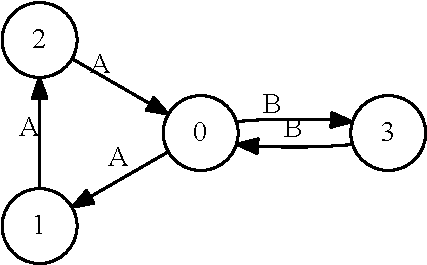
\includegraphics[width=6cm]{dot/input.pdf}
        \caption{The map of School (input graph $M$)}
        \label{input}        
    \end{center}
\end{figure}


And now you want to find the path from your current position to the same floor of another tower. 
Map with all such paths can help you.
But orienting is not your forte, so it would be great if all structure of paths will be ass simple as possible and all paths will have checkpoints to control your rout.

It is evident that one of simplest structure of required paths is $\{ab, aabb, aaabbb, \dots\}$.
In terms of our definitions you have a graph $M=(\{0;1;2;3\},E,\{a;b\})$ (figure~\ref{input}), and you want to find all paths $p$, such that $\Omega(p) \in \{ab; aabb; aaabbb; \dots\}$ or $\Omega(p) \in a^n b^n$ where $n \geq 1$.


First problem is that language $\mathcal{L} = \{a^n b^n; n \geq 1\}$ is not a regular and this fact restricts the set of tools which you can use. 
Another problem is that solution in presented case is an infinite set of path, and you want to get a finite map without any magic.  
Moreover, you want to know a structure of paths with checkpoints added.

We do not know any existing tools which can help to solve your problem and we create a new one.
Let us to show how to get the map which help to orient in this strange School.

Fortunately the language $\mathcal{L} = \{a^n b^n; n \geq 1\}$ is a context-free language and can be specified by context-free grammar. 
The fact that one language can be described with more then one grammar allow you to add checkpoints: you can use additional nonterminals for ``marking'' required parts of sentence.
In our case the good checkpoint is a middle of path.
As a result, required language can be specified by grammar $G_1$ presented in picture~\ref{grammarG} where $N = \{s; \text{\textit{Middle}}\}$, $\Sigma = \{a; b\}$, and $S$ is a start nonterminal.

\begin{figure}[h]
   \begin{center}
   \[
\begin{array}{rl}
   0:& S \rightarrow a \ S \ b \\
   1:& S \rightarrow Middle \\
   2:& Middle \rightarrow a \ b
\end{array}
\]

   \caption{Grammar $G_1$ for language $L=\{a^n b^n; n \geq 1\}$ with additional marker for path's middle}
   \label{grammarG}        
   \end{center}
\end{figure}

Algorithm of map construction is presented below.
